
%% bare_conf.tex
%% V1.3
%% 2007/01/11
%% by Michael Shell
%% See:
%% http://www.michaelshell.org/
%% for current contact information.
%%
%% This is a skeleton file demonstrating the use of IEEEtran.cls
%% (requires IEEEtran.cls version 1.7 or later) with an IEEE conference paper.
%%
%% Support sites:
%% http://www.michaelshell.org/tex/ieeetran/
%% http://www.ctan.org/tex-archive/macros/latex/contrib/IEEEtran/
%% and
%% http://www.ieee.org/

%%*************************************************************************
%% Legal Notice:
%% This code is offered as-is without any warranty either expressed or
%% implied; without even the implied warranty of MERCHANTABILITY or
%% FITNESS FOR A PARTICULAR PURPOSE!
%% User assumes all risk.
%% In no event shall IEEE or any contributor to this code be liable for
%% any damages or losses, including, but not limited to, incidental,
%% consequential, or any other damages, resulting from the use or misuse
%% of any information contained here.
%%
%% All comments are the opinions of their respective authors and are not
%% necessarily endorsed by the IEEE.
%%
%% This work is distributed under the LaTeX Project Public License (LPPL)
%% ( http://www.latex-project.org/ ) version 1.3, and may be freely used,
%% distributed and modified. A copy of the LPPL, version 1.3, is included
%% in the base LaTeX documentation of all distributions of LaTeX released
%% 2003/12/01 or later.
%% Retain all contribution notices and credits.
%% ** Modified files should be clearly indicated as such, including  **
%% ** renaming them and changing author support contact information. **
%%
%% File list of work: IEEEtran.cls, IEEEtran_HOWTO.pdf, bare_adv.tex,
%%                    bare_conf.tex, bare_jrnl.tex, bare_jrnl_compsoc.tex
%%*************************************************************************

% *** Authors should verify (and, if needed, correct) their LaTeX system  ***
% *** with the testflow diagnostic prior to trusting their LaTeX platform ***
% *** with production work. IEEE's font choices can trigger bugs that do  ***
% *** not appear when using other class files.                            ***
% The testflow support page is at:
% http://www.michaelshell.org/tex/testflow/



% Note that the a4paper option is mainly intended so that authors in
% countries using A4 can easily print to A4 and see how their papers will
% look in print - the typesetting of the document will not typically be
% affected with changes in paper size (but the bottom and side margins will).
% Use the testflow package mentioned above to verify correct handling of
% both paper sizes by the user's LaTeX system.
%
% Also note that the "draftcls" or "draftclsnofoot", not "draft", option
% should be used if it is desired that the figures are to be displayed in
% draft mode.
%
\documentclass[conference]{IEEEtran}
% Add the compsoc option for Computer Society conferences.
%
% If IEEEtran.cls has not been installed into the LaTeX system files,
% manually specify the path to it like:
% \documentclass[conference]{../sty/IEEEtran}





% Some very useful LaTeX packages include:
% (uncomment the ones you want to load)


% *** MISC UTILITY PACKAGES ***
%
%\usepackage{ifpdf}
% Heiko Oberdiek's ifpdf.sty is very useful if you need conditional
% compilation based on whether the output is pdf or dvi.
% usage:
% \ifpdf
%   % pdf code
% \else
%   % dvi code
% \fi
% The latest version of ifpdf.sty can be obtained from:
% http://www.ctan.org/tex-archive/macros/latex/contrib/oberdiek/
% Also, note that IEEEtran.cls V1.7 and later provides a builtin
% \ifCLASSINFOpdf conditional that works the same way.
% When switching from latex to pdflatex and vice-versa, the compiler may
% have to be run twice to clear warning/error messages.






% *** CITATION PACKAGES ***
%
%\usepackage{cite}
% cite.sty was written by Donald Arseneau
% V1.6 and later of IEEEtran pre-defines the format of the cite.sty package
% \cite{} output to follow that of IEEE. Loading the cite package will
% result in citation numbers being automatically sorted and properly
% "compressed/ranged". e.g., [1], [9], [2], [7], [5], [6] without using
% cite.sty will become [1], [2], [5]--[7], [9] using cite.sty. cite.sty's
% \cite will automatically add leading space, if needed. Use cite.sty's
% noadjust option (cite.sty V3.8 and later) if you want to turn this off.
% cite.sty is already installed on most LaTeX systems. Be sure and use
% version 4.0 (2003-05-27) and later if using hyperref.sty. cite.sty does
% not currently provide for hyperlinked citations.
% The latest version can be obtained at:
% http://www.ctan.org/tex-archive/macros/latex/contrib/cite/
% The documentation is contained in the cite.sty file itself.






% *** GRAPHICS RELATED PACKAGES ***
%
  \usepackage{graphicx}
  \usepackage{verbatim}
   \usepackage{url}
   \usepackage{flushend}

\ifCLASSINFOpdf
  % \usepackage[pdftex]{graphicx}
  % declare the path(s) where your graphic files are
  % \graphicspath{{../pdf/}{../jpeg/}}
  % and their extensions so you won't have to specify these with
  % every instance of \includegraphics
  % \DeclareGraphicsExtensions{.pdf,.jpeg,.png}
\else
  % or other class option (dvipsone, dvipdf, if not using dvips). graphicx
  % will default to the driver specified in the system graphics.cfg if no
  % driver is specified.
  % \usepackage[dvips]{graphicx}
  % declare the path(s) where your graphic files are
  % \graphicspath{{../eps/}}
  % and their extensions so you won't have to specify these with
  % every instance of \includegraphics
  % \DeclareGraphicsExtensions{.eps}
\fi
% graphicx was written by David Carlisle and Sebastian Rahtz. It is
% required if you want graphics, photos, etc. graphicx.sty is already
% installed on most LaTeX systems. The latest version and documentation can
% be obtained at:
% http://www.ctan.org/tex-archive/macros/latex/required/graphics/
% Another good source of documentation is "Using Imported Graphics in
% LaTeX2e" by Keith Reckdahl which can be found as epslatex.ps or
% epslatex.pdf at: http://www.ctan.org/tex-archive/info/
%
% latex, and pdflatex in dvi mode, support graphics in encapsulated
% postscript (.eps) format. pdflatex in pdf mode supports graphics
% in .pdf, .jpeg, .png and .mps (metapost) formats. Users should ensure
% that all non-photo figures use a vector format (.eps, .pdf, .mps) and
% not a bitmapped formats (.jpeg, .png). IEEE frowns on bitmapped formats
% which can result in "jaggedy"/blurry rendering of lines and letters as
% well as large increases in file sizes.
%
% You can find documentation about the pdfTeX application at:
% http://www.tug.org/applications/pdftex





% *** MATH PACKAGES ***
%
%\usepackage[cmex10]{amsmath}
% A popular package from the American Mathematical Society that provides
% many useful and powerful commands for dealing with mathematics. If using
% it, be sure to load this package with the cmex10 option to ensure that
% only type 1 fonts will utilized at all point sizes. Without this option,
% it is possible that some math symbols, particularly those within
% footnotes, will be rendered in bitmap form which will result in a
% document that can not be IEEE Xplore compliant!
%
% Also, note that the amsmath package sets \interdisplaylinepenalty to 10000
% thus preventing page breaks from occurring within multiline equations. Use:
%\interdisplaylinepenalty=2500
% after loading amsmath to restore such page breaks as IEEEtran.cls normally
% does. amsmath.sty is already installed on most LaTeX systems. The latest
% version and documentation can be obtained at:
% http://www.ctan.org/tex-archive/macros/latex/required/amslatex/math/





% *** SPECIALIZED LIST PACKAGES ***
%
%\usepackage{algorithmic}
% algorithmic.sty was written by Peter Williams and Rogerio Brito.
% This package provides an algorithmic environment fo describing algorithms.
% You can use the algorithmic environment in-text or within a figure
% environment to provide for a floating algorithm. Do NOT use the algorithm
% floating environment provided by algorithm.sty (by the same authors) or
% algorithm2e.sty (by Christophe Fiorio) as IEEE does not use dedicated
% algorithm float types and packages that provide these will not provide
% correct IEEE style captions. The latest version and documentation of
% algorithmic.sty can be obtained at:
% http://www.ctan.org/tex-archive/macros/latex/contrib/algorithms/
% There is also a support site at:
% http://algorithms.berlios.de/index.html
% Also of interest may be the (relatively newer and more customizable)
% algorithmicx.sty package by Szasz Janos:
% http://www.ctan.org/tex-archive/macros/latex/contrib/algorithmicx/




% *** ALIGNMENT PACKAGES ***
%
%\usepackage{array}
% Frank Mittelbach's and David Carlisle's array.sty patches and improves
% the standard LaTeX2e array and tabular environments to provide better
% appearance and additional user controls. As the default LaTeX2e table
% generation code is lacking to the point of almost being broken with
% respect to the quality of the end results, all users are strongly
% advised to use an enhanced (at the very least that provided by array.sty)
% set of table tools. array.sty is already installed on most systems. The
% latest version and documentation can be obtained at:
% http://www.ctan.org/tex-archive/macros/latex/required/tools/


%\usepackage{mdwmath}
%\usepackage{mdwtab}
% Also highly recommended is Mark Wooding's extremely powerful MDW tools,
% especially mdwmath.sty and mdwtab.sty which are used to format equations
% and tables, respectively. The MDWtools set is already installed on most
% LaTeX systems. The lastest version and documentation is available at:
% http://www.ctan.org/tex-archive/macros/latex/contrib/mdwtools/


% IEEEtran contains the IEEEeqnarray family of commands that can be used to
% generate multiline equations as well as matrices, tables, etc., of high
% quality.


%\usepackage{eqparbox}
% Also of notable interest is Scott Pakin's eqparbox package for creating
% (automatically sized) equal width boxes - aka "natural width parboxes".
% Available at:
% http://www.ctan.org/tex-archive/macros/latex/contrib/eqparbox/





% *** SUBFIGURE PACKAGES ***
%\usepackage[tight,footnotesize]{subfigure}
% subfigure.sty was written by Steven Douglas Cochran. This package makes it
% easy to put subfigures in your figures. e.g., "Figure 1a and 1b". For IEEE
% work, it is a good idea to load it with the tight package option to reduce
% the amount of white space around the subfigures. subfigure.sty is already
% installed on most LaTeX systems. The latest version and documentation can
% be obtained at:
% http://www.ctan.org/tex-archive/obsolete/macros/latex/contrib/subfigure/
% subfigure.sty has been superceeded by subfig.sty.



%\usepackage[caption=false]{caption}
%\usepackage[font=footnotesize]{subfig}
% subfig.sty, also written by Steven Douglas Cochran, is the modern
% replacement for subfigure.sty. However, subfig.sty requires and
% automatically loads Axel Sommerfeldt's caption.sty which will override
% IEEEtran.cls handling of captions and this will result in nonIEEE style
% figure/table captions. To prevent this problem, be sure and preload
% caption.sty with its "caption=false" package option. This is will preserve
% IEEEtran.cls handing of captions. Version 1.3 (2005/06/28) and later
% (recommended due to many improvements over 1.2) of subfig.sty supports
% the caption=false option directly:
%\usepackage[caption=false,font=footnotesize]{subfig}
%
% The latest version and documentation can be obtained at:
% http://www.ctan.org/tex-archive/macros/latex/contrib/subfig/
% The latest version and documentation of caption.sty can be obtained at:
% http://www.ctan.org/tex-archive/macros/latex/contrib/caption/




% *** FLOAT PACKAGES ***
%
%\usepackage{fixltx2e}
% fixltx2e, the successor to the earlier fix2col.sty, was written by
% Frank Mittelbach and David Carlisle. This package corrects a few problems
% in the LaTeX2e kernel, the most notable of which is that in current
% LaTeX2e releases, the ordering of single and double column floats is not
% guaranteed to be preserved. Thus, an unpatched LaTeX2e can allow a
% single column figure to be placed prior to an earlier double column
% figure. The latest version and documentation can be found at:
% http://www.ctan.org/tex-archive/macros/latex/base/



%\usepackage{stfloats}
% stfloats.sty was written by Sigitas Tolusis. This package gives LaTeX2e
% the ability to do double column floats at the bottom of the page as well
% as the top. (e.g., "\begin{figure*}[!b]" is not normally possible in
% LaTeX2e). It also provides a command:
%\fnbelowfloat
% to enable the placement of footnotes below bottom floats (the standard
% LaTeX2e kernel puts them above bottom floats). This is an invasive package
% which rewrites many portions of the LaTeX2e float routines. It may not work
% with other packages that modify the LaTeX2e float routines. The latest
% version and documentation can be obtained at:
% http://www.ctan.org/tex-archive/macros/latex/contrib/sttools/
% Documentation is contained in the stfloats.sty comments as well as in the
% presfull.pdf file. Do not use the stfloats baselinefloat ability as IEEE
% does not allow \baselineskip to stretch. Authors submitting work to the
% IEEE should note that IEEE rarely uses double column equations and
% that authors should try to avoid such use. Do not be tempted to use the
% cuted.sty or midfloat.sty packages (also by Sigitas Tolusis) as IEEE does
% not format its papers in such ways.





% *** PDF, URL AND HYPERLINK PACKAGES ***
%
%\usepackage{url}
% url.sty was written by Donald Arseneau. It provides better support for
% handling and breaking URLs. url.sty is already installed on most LaTeX
% systems. The latest version can be obtained at:
% http://www.ctan.org/tex-archive/macros/latex/contrib/misc/
% Read the url.sty source comments for usage information. Basically,
% \url{my_url_here}.





% *** Do not adjust lengths that control margins, column widths, etc. ***
% *** Do not use packages that alter fonts (such as pslatex).         ***
% There should be no need to do such things with IEEEtran.cls V1.6 and later.
% (Unless specifically asked to do so by the journal or conference you plan
% to submit to, of course. )


% correct bad hyphenation here
\hyphenation{op-tical net-works semi-conduc-tor}


\begin{document}

%
% paper title
% can use linebreaks \\ within to get better formatting as desired
\title{Ontology Development in EEG/ERP Portal}


% author names and affiliations
% use a multiple column layout for up to three different
% affiliations
\author{\IEEEauthorblockN{Petr Je\v{z}ek, Roman Mou\v{c}ek}
\IEEEauthorblockA{
Department of Computer Science and Engineering, \\
University of West Bohemia, \\
Pilsen, Czech Republic\\
}
}

% conference papers do not typically use \thanks and this command
% is locked out in conference mode. If really needed, such as for
% the acknowledgment of grants, issue a \IEEEoverridecommandlockouts
% after \documentclass

% for over three affiliations, or if they all won't fit within the width
% of the page, use this alternative format:
%
%\author{\IEEEauthorblockN{Michael Shell\IEEEauthorrefmark{1},
%Homer Simpson\IEEEauthorrefmark{2},
%James Kirk\IEEEauthorrefmark{3},
%Montgomery Scott\IEEEauthorrefmark{3} and
%Eldon Tyrell\IEEEauthorrefmark{4}}
%\IEEEauthorblockA{\IEEEauthorrefmark{1}School of Electrical and Computer Engineering\\
%Georgia Institute of Technology,
%Atlanta, Georgia 30332--0250}
%\IEEEauthorblockA{\IEEEauthorrefmark{2}Twentieth Century Fox, Springfield, USA}
%\IEEEauthorblockA{\IEEEauthorrefmark{3}Starfleet Academy, San Francisco, California 96678-2391\\
%Telephone: (800) 555--1212, Fax: (888) 555--1212}
%\IEEEauthorblockA{\IEEEauthorrefmark{4}Tyrell Inc., 123 Replicant Street, Los Angeles, California 90210--4321}}




% use for special paper notices
%\IEEEspecialpapernotice{(Invited Paper)}




% make the title area
\maketitle


\begin{abstract}
%\boldmath
Substantial difficulties related to collecting data/metadata from EEG/ERP experiments are presented. Since a suitable ontology describing EEG/ERP experiments does not exist, authors present a custom ontology that is proposed to be discussed within the scientific community. The presented ontology is practically implemented within the EEG/ERP Portal. The EEG/ERP Portal simultaneously serves to interested community as a tool for sharing and managing custom EEG/ERP experiments. Since domain ontologies are expressed by the Semantic Web languages (OWL), authors present a brief introduction into the Semantic Web technologies. Semantic Web languages expressivity is different in contrast with the object-oriented code that is most often used in current software development. The developed Semantic Framework ensures adding missing semantics into the input object-oriented code and its transformation into appropriate OWL constructs. Integration of the Semantic Framework into the EEG/ERP Portal ensures an online serialization of stored experiments into an OWL document. Registration of the developed ontology in NIF validates authors' approach. The NIF registration also enables easy sharing of stored experiments.
\end{abstract}
% IEEEtran.cls defaults to using nonbold math in the Abstract.
% This preserves the distinction between vectors and scalars. However,
% if the conference you are submitting to favors bold math in the abstract,
% then you can use LaTeX's standard command \boldmath at the very start
% of the abstract to achieve this. Many IEEE journals/conferences frown on
% math in the abstract anyway.

\begin{IEEEkeywords}
neuroinformatics, electroencephalography, event-related potentials, data management, Semantic Web, Semantic Framework, EEG/ERP experiment, EEG/ERP Portal, ontology
\end{IEEEkeywords}




% For peer review papers, you can put extra information on the cover
% page as needed:
% \ifCLASSOPTIONpeerreview
% \begin{center} \bfseries EDICS Category: 3-BBND \end{center}
% \fi
%
% For peerreview papers, this IEEEtran command inserts a page break and
% creates the second title. It will be ignored for other modes.
\IEEEpeerreviewmaketitle



\section{Introduction}

Our research group at University of West Bohemia in Pilsen specializes in the research of brain activity. We use the methods of Electroencephalography (EEG) and its derived technique Event-Related Potentials (ERP). EEG/ERP experiments are time-consuming performed in a specially equipped laboratory. With the increasing number of experiments we were facing the problem with their long-term storage and management.

We are a member of the Czech National Node of International Neuroscience Coordinating Facility (INCF) that is concerned with the organization of neuroscience data,
application of computational models and analytical tools, etc. One of the objectives of INCF is to define standardized formats and  an infrastructure for neurophysiological research. Our aim within the INCF is to provide a complete technological support for storing and sharing EEG/ERP experiments.

Despite a lot of tools that are being developed, potential benefits that the dissemination of knowledge among laboratories offers are still not used. The main reason is that the medical software is supplied by various mostly commercial vendors who are not interested in developing reusable standards. On the other hand, the suitable medium for sharing experimental data should be the Internet. Despite the popularity of the Internet, how it is growing, it contains a huge amount of information with practically no classification. Such not classified data are not suitable for sharing. As a solution an extension called the Semantic Web that is intended to give the data semantic meaning is being developed. Despite of advantages that the Semantic Web brings commonly used systems are usually object oriented.

Since semantic gaps between common modeling techniques and the Semantic Web exist, we needed to describe the most serious of them and investigate their removal. We present the proposed mapping and its implementation that extends a common object oriented code by missing semantics. The proposed mapping was practically implemented within a custom Semantic Framework.

The ontology that precisely describes the EEG/ERP experiment is presented. Our effort to provide a system for storing and management of EEG/ERP experiments resulted in a custom solution called the EEG/ERP Portal. The developed Semantic Framework generates experimental ontology from the EEG/ERP Portal that is integrated within the NIF registry.

\section{EEG/ERP Experiments}

\subsection{Introduction}

EEG/ERP is a technique for recording and interpreting the electrical activity of the brain. This technique is widely used in the research of the brain activity (e. g. reaction of comatose patients, monitoring of drivers' attention, etc.). We perform experiments based on classical oddball paradigm \cite{Introduction-to-ERP}. Such experiments typically contain two stimuli.
Stimuli are presented in a random series such that one of them occurs relatively infrequently. The first one presented more often is called non-target and the second one is called target. The tested subject is instructed to be concentrated on the target stimuli. Simple signal averaging procedure is performed continuously during the session after each stimulus subside. Averaging extracts the ERPs from the signal.

\subsection{\label{Difficulties}Difficulties}

Since data obtained during EEG/ERP experiments are raw data, we need to extend them by metadata description. Data/metadata have to be further processable by software tools. It includes searching, interchanging or managing. Data/metadata are usually stored in a relational database. On the other hand, tools that
work with data/metadata are usually based on the object oriented programming. Such stored data/metadata can be expressed by the Semantic Web languages to be searchable by automatic readers. Each approach uses a different way to access them. Because of different possibilities for expressing a semantic meaning of data a need of suitable mapping is emerging.

\subsection{\label{Experimental Ontology}Experimental Ontology}

Since description of the EEG/ERP experiments is desirable we propose a custom ontology that precisely describes this domain.

When data from experiments are described by suitable metadata in a well-formed structure they may be reproduced and processed across laboratories.

The specification of the ontology originated from experience of our laboratory, co-workers from cooperating institutions, books describing principles of EEG/ERP design and data recording (e.g. \cite{Introduction-to-ERP}) and numerous scientific papers describing specific EEG/ERP experiments. It also corresponds to the effort of the INCF \cite{incf-sustainability-report} in the field of development and standardization of databases in neuroinformatics.

Experimental data are supplemented by its description according to a defined protocol. The collected metadata can be divided into several semantic groups according to their semantic meaning. We defined the following semantic groups:

\emph{Activity} - describes the activity that takes place according to the specific scenario. It includes information about video, pictures on the computer screen, sound sloughed off into the headphones, or information about the instructions that received the tested subject when the experiment started. The description of stimuli is also present.

\emph{Environment} - describes surrounding conditions. It includes weather, time of the day, and temperature.

\emph{Tested subject} - describes information about the tested subject. It includes laterality, education, age, gender, diseases, disability, and medications.

\emph{Hardware equipment} - describes the type, producer and the serial number of the used hardware.

\emph{Software equipment} - describes software that was used during the experiment. It includes the name of the software, version, producer, and configuration files if they are used.

\emph{Used electrodes} - describes the type, impedance, location, used system, and fixation of used electrodes.

\emph{Signal digitalization} - describes a set of parameters that influence conversion of data using a specific analogue-digital converter. It includes filtration, sampling frequency, and band-pass.

\emph{Signal analysis} - describes the technique of analyzing the EEG/ERP signal. It includes the length of pre- and post- stimuli part of the signal, the number of epochs and the verbal description of signal processing procedure.

\emph{Data presentation} - describes experimental results or assumptions needed to reproduce the experiment. It includes Averaged ERP waves, grand averages, evolution of ERP in time and space, waves description (a description of the well-known or new waves which were formed during study), link to raw experimental data (a link to all recorded raw data).

\emph{Artifact} - Artifacts may originate from muscle activities, eyes movement, etc. It contains information describing a compensation method that prevents the formation of the artifact. When a method for removing of the formed artifact is used, the description is also placed there. When some artifact totally degrades the signal, the user can define conditions when it is possible to assume the signal as totally useless.

\section{\label{EEG/ERP Portal}EEG/ERP Portal}

\subsection{Context}

Because of hard manual work with large amounts of EEG/ERP data and metadata, and difficulties mentioned in \ref{Difficulties}, we decided to design and implement a custom software tool suitable for EEG/ERP data and metadata storage and management. As the result we developed the system called the EEG/ERP Portal intended not only for our local research. In general, it  contributes to advancements in human brain understanding.

The interpretation of EEG/ERP experimental data/metadata is solved by developing a custom ontology described in \ref{Experimental Ontology}. The practical implementation of the designed ontology is ensured by the database structure and the internal logic of the developed EEG/ERP Portal. The EEG/ERP Portal provides a possibility to store, get, manage or interchange
EEG/ERP experiments among interested researchers. The internal data storage structure is implemented according to the developed ontology.

Several additional modules are also implemented. It includes a module for interaction within social networks, a library of analytical tools, a semantic web module or web services for interaction with other systems.

\subsection{Architecture}

The EEG/ERP Portal is web based application. It uses three-layer architecture. This architectonic style is supported by selection of programming tools and technologies. We used Java
and XML technologies to ensure a high level of abstraction (system extensibility) as well as a long term existence of the EEG/ERP Portal as open source.

\subsubsection{Persistence Layer}

The persistence layer uses the Hibernate framework. It means that a relational database and an object - relational mapping are supported. Oracle 11g database server is used to ensure the processing of large data files.

\subsubsection{Application and Presentation Layers}

The application and presentation layers are designed and implemented using the Spring technology. This framework supports MVC architecture, dependency
injection and aspect oriented programming. The Spring Security framework is used to ensure management of authentication and user roles. User access to the system is realized through the web interface. Majority of users are familiarized with web applications and they do not need any additional software except a web browser. The user interface is divided into several parts (the main menu, the second level menu, the header, the footer and a content part). Figure \ref{fig:EEG/ERP Portal Preview} shows the preview of the EEG/ERP Portal.

\begin{figure}[h]
	\centering
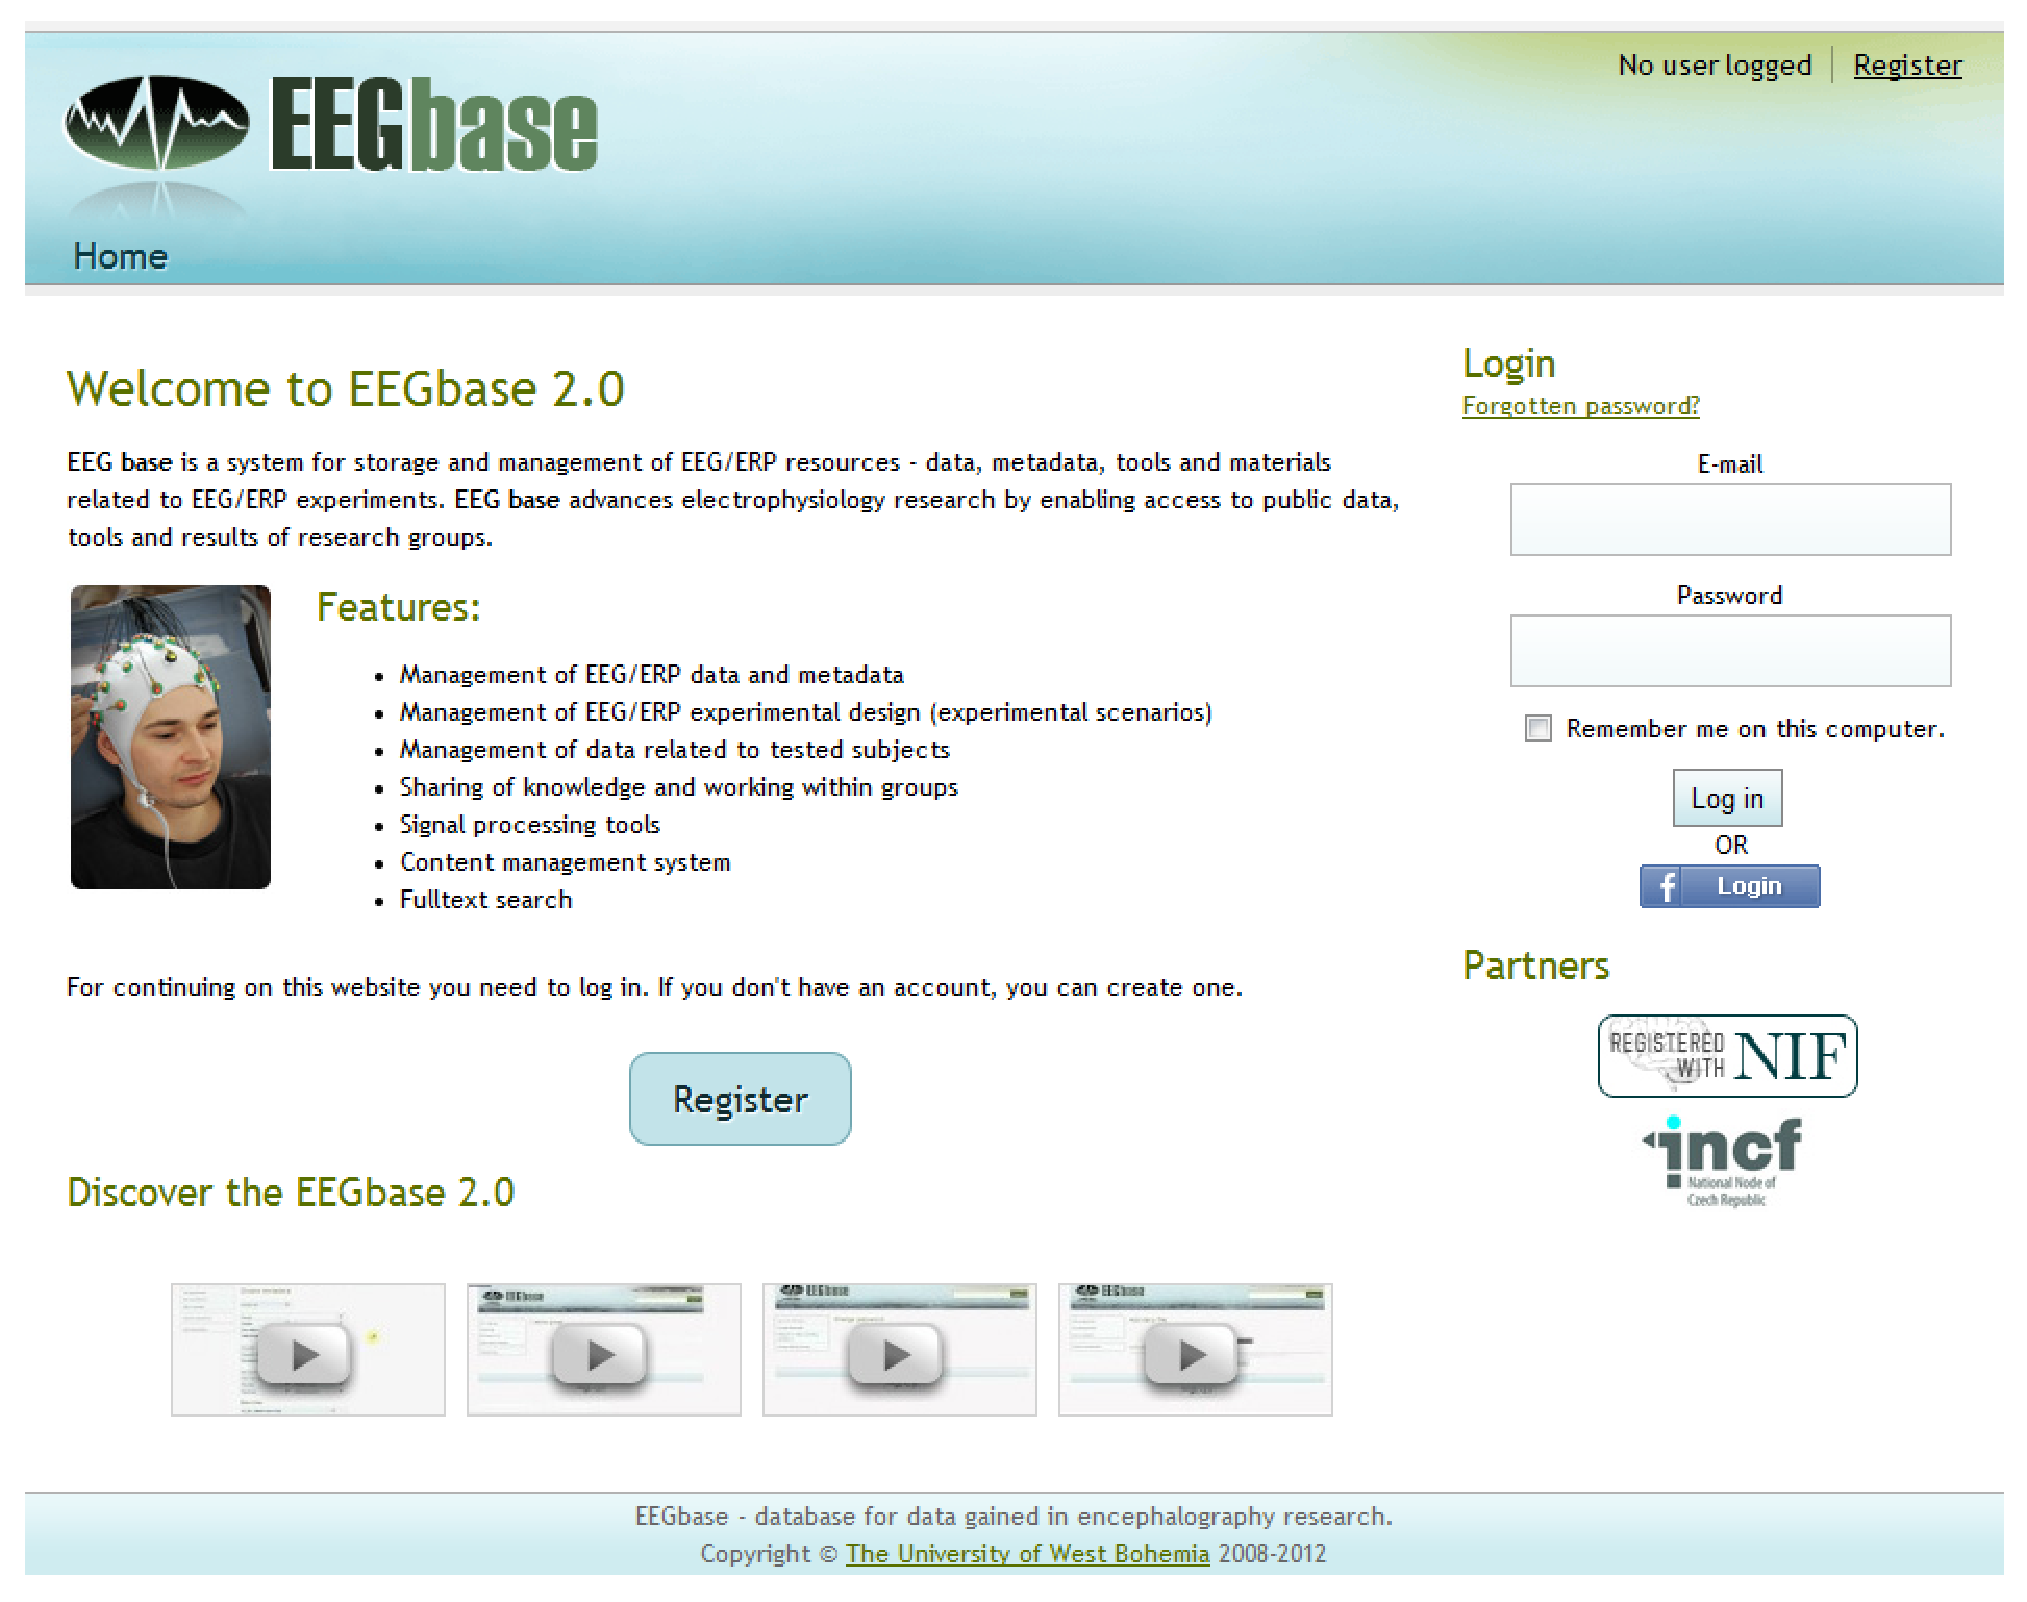
\includegraphics[scale=0.24]{eeg_erp_portal_preview}

\caption{\label{fig:EEG/ERP Portal Preview}EEG/ERP Portal Preview}

\end{figure}


\section{Semantic Web Technologies}

\subsection{RDF and OWL}

The Semantic Web is a layered architecture. The first layer is called Resource Description Framework (RDF). RDF is a simple metadata representation framework, using URIs to identify web-based resources and a graph model for describing relationships between resources.

Web ontology language (OWL) is a richer language and provides more complex constraints on the types of resources and their properties. OWL comes with a larger vocabulary, greater machine interpretability, and stronger syntax than RDF. Because of  richer semantic expressivity and needs that the registration in NIF (see \ref{Registration within NIF}) requires, we decided to transform data/metadata from the EEG/ERP Portal into OWL.

\subsection{OOP to OWL Mapping}

A description of similar and different concepts of OOP (expressed by UML diagrams) and OWL expressions is given.

\subsubsection{Similar Concepts}

Both OWL and UML are based on classes. Relationships among OWL classes are called \emph{properties}. Properties are not necessarily tied to a specific class. The UML properties are translated to \emph{owl:ObjectProperty} if the type of Property is UML Class and \emph{owl:DatatypeProperty} otherwise. Both support a separation into modules, called \emph{package} in UML and \emph{ontology} in OWL. Both support fixed enumeration of elements. Both languages allow the class to be a subclass of more than one class. OWL properties can be constrained by cardinality restrictions. UML also supports cardinality restrictions.

\subsubsection{Different Concepts}

In the common OOP the names within one namespace always refer to the same object, and different names always refer to a different object (unique name assumption). Names in OWL do not by default fulfill unique name assumption. Facilities of UML for supporting programs include \emph{operations}, \emph{responsibilities}, \emph{static operations}, \emph{interface classes}, \emph{abstract classes}. In contrast OWL is intended to only represent data and additional data semantics that enables to infer an additional data meaning \cite{ODM}.


\subsection{\label{Existing Tools}Existing Tools}

We tested several tools that transform common object oriented code into the Semantic Web languages. The most of tested tools are based on Jena \cite{Jena}. It provides a program environment
for RDF, RDFS, OWL, SparQL languages and technologies.

Mapping of OWL classes to Java Interfaces is described in \cite{mapping-owl-into-java}. Every OWL class is mapped into a Java Interface containing just the accessor/mutator method declarations (set/get methods) for properties of that class.

Back transformation is described in \cite{owl-vs-oop} where an OWL processor SWCLOS3 is developed. It is on top of Common Lisp Object System (CLOS). It allows lisp programmers to construct domain and task ontologies in software application fields.

Java2OWL-S is a tool which is able to generate OWL directly \cite{java2owl}. It uses two transformation. The first one transforms a java code into a temporary WSDL file. The second one transforms this file into an OWL.

JenaBean \cite{JenaBean} is a similar tool; it is a flexible RDF/OWL API to persist JavaBeans. It takes an approach to binding that is driven by the Java object model rather than the OWL or RDF schema.

Concerning one side transformations the tools above work quite satisfactorily because object-oriented code has poorer semantics than OWL. However, if we want to use more capabilities of OWL, enrichment of object-oriented code by missing semantics is needed.

The ActiceRDF \cite{ActiveRDF} is a library for accessing RDF data from Ruby programs. It provides a domain specific language for RDF models; it can address
RDF resources, classes and properties programmatically.

The Semantic object framework (SOF) \cite{SOF} utilizes embedded comments in source codes to describe semantic relationships between classes and attributes.

The eClass \cite{Web-Information-Representation} is a solution that changes Java syntax to embed semantic descriptions into the source code.

\section{Semantic Framework}

\subsection{Context}

According to Subsection \ref{Difficulties} the mapping from a common object-oriented code is not successfully solved.

  \begin{figure*}[t!]
	\centering
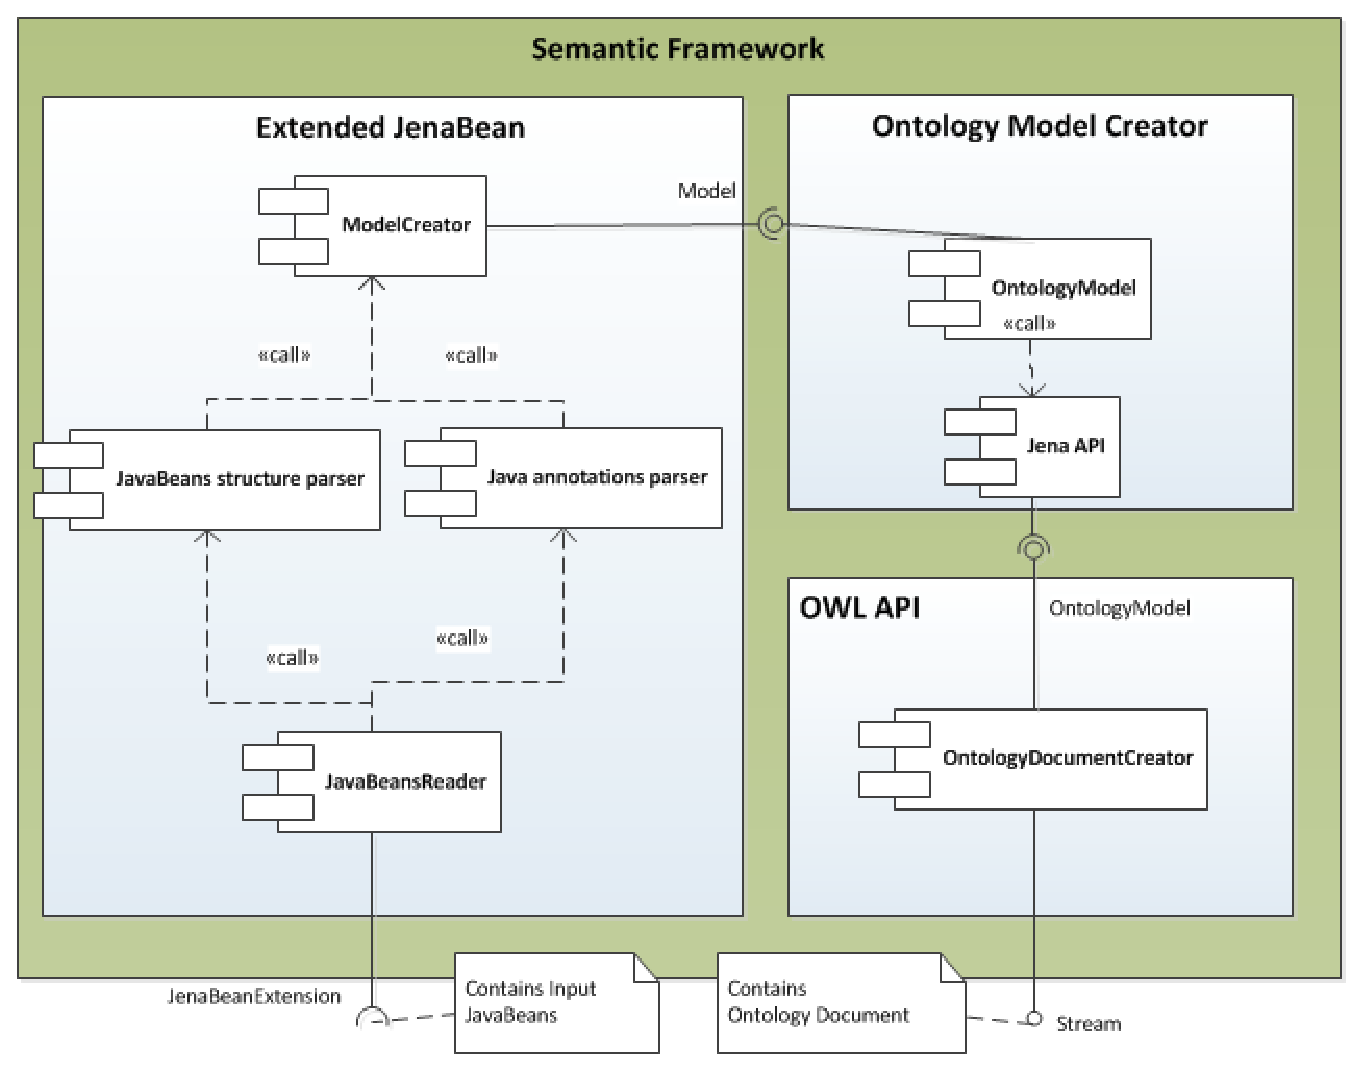
\includegraphics[width=12cm, height=8cm]{SemanticFramework_Component_Model}

\caption{\label{fig:Component Diagram of Semantic Framework}Component Diagram of Semantic Framework}

\end{figure*}

The tools described in Subsection \ref{Existing Tools} are able to transform only common semantics including classes definitions and its properties.

Some of tested frameworks try to enrich the input object-oriented code by missing semantics using either embedded comments or changing the JavaBean syntax. The usage of such tools is difficult  because it requires a modified compiler and java interpreter. Because of the EEG/ERP Portal works with the data stored in common JavaBeans as well, we decided to propose a mapping that enables adding missing semantics into the common JavaBean structure. The extension of the common JavaBean structure is based on the idea we initially presented in \cite{Transformation-of-object-oriented-code-into-semantic-web-using-Java-annotations}. The complete set of proposed annotations and its mapping to appropriate OWL constructs is described in \cite{Semantic-Web-in-EEG-ERP-Portal}.


\subsection{Implementation}

The Semantic Framework is provided as a library that user can integrate into a custom system. The input is a set of JavaBeans and the output is an ontology document. The ontology document can be serialized into the several supported Semantic Web languages syntaxes. We currently support RDF/XML, OWL/XML, Turtle, Abbreviated OWL/XML formats.

Figure \ref{fig:Component Diagram of Semantic Framework} shows the component diagram of the Semantic Framework. The framework contains three main subcomponents. The first subcomponent is the modified JenaBean. We extend the current JenaBean so that the output corresponds to the proposed mapping. Moreover, we added the processing of Java annotations into the processing of JavaBeans structure so we are able to transform the set of proposed annotations. The output of the extended JenaBean component is an internal model representation.


This internal model representation is submitted to the second, Ontology Model Creator, subcomponent. This subcomponent creates an Ontology model using an Ontology Model Factory. The internal JenaBean model is processed and an ontology document is created by calling Jena API methods. The result model can be further processed by the last subcomponent, OWL API, that transforms an ontology model into the supported ontology formats.


\subsection{Integration within EEG/ERP Portal}

The input point of the EEG/ERP Portal internal logic is created by the set of controllers according to Spring MVC design. The controllers process a HTTP requests and generate a related response. We defined a set of URLs processed by a \emph{SemanticMultiController} that processes an OWL reasoner request. The controller contains methods for getting an OWL document in the supported syntaxes.

When the \emph{SemanticMultiController} processes input parameters, it calls a \emph{SemanticFactory} interface. This factory is responsible for getting JavaBeans from the database and handover them to the \emph{Semantic Framework}. When the \emph{Semantic Framework} gets the ontology document, it returns a \emph{Data Stream} back to the web browser.

The Semantic Framework is controlled by a build-in timer. The timer calls the Semantic Framework API in regular intervals. It generates the ontology document and stores it into a temporary file. When any document request appears, the temporary file containing the actual set of stored experiments is immediately available. This approach ensures a quick response because the ontology document is pre-prepared.


\section{\label{Registration within NIF}Registration within NIF}

\subsection{Introduction}

NIF is a portal that serves as an online inventory of registered neuroscience data sources. Since the NIF is important framework within the INCF community developed according to INCF recommendations \cite{incf-sustainability-report} we have choose it as the best choice for validating the developed ontology.

\subsection{Static Context Registration}

NIF uses a proprietary framework \emph{Disco} \cite{NIF-Neuroinformatics}. The registered resource is described using two XML files: \emph{disco.xml} and \emph{disco.rd.xml}. Both have RDF syntax so they are computer-processable on the NIF side. The first file provides a basic description of the registered resource as its URL, contact, etc. The second one provides a more detailed description of the source as a description of partial sections of the system, keywords, publication links, etc. These files are located in the root of our EEG/ERP Portal so they are accessible by the NIF automatic readers.

\subsection{Dynamic Context Registration}

The dynamic content of the EEG/ERP Portal is accessed by the proprietary NIF protocol \emph{Interoperability XML} \cite{ncbo-bioPortal}. The Interoperability XML is used to describe the structure of metadata instances stored in the ontology document. NIF reloads it in regular intervals. When the \emph{Interoperability XML} file is reloaded the ontology document is reloaded as well.

% An example of a floating figure using the graphicx package.
% Note that \label must occur AFTER (or within) \caption.
% For figures, \caption should occur after the \includegraphics.
% Note that IEEEtran v1.7 and later has special internal code that
% is designed to preserve the operation of \label within \caption
% even when the captionsoff option is in effect. However, because
% of issues like this, it may be the safest practice to put all your
% \label just after \caption rather than within \caption{}.
%
% Reminder: the "draftcls" or "draftclsnofoot", not "draft", class
% option should be used if it is desired that the figures are to be
% displayed while in draft mode.
%
%\begin{figure}[!t]
%\centering
%\includegraphics[width=2.5in]{myfigure}
% where an .eps filename suffix will be assumed under latex,
% and a .pdf suffix will be assumed for pdflatex; or what has been declared
% via \DeclareGraphicsExtensions.
%\caption{Simulation Results}
%\label{fig_sim}
%\end{figure}

% Note that IEEE typically puts floats only at the top, even when this
% results in a large percentage of a column being occupied by floats.


% An example of a double column floating figure using two subfigures.
% (The subfig.sty package must be loaded for this to work.)
% The subfigure \label commands are set within each subfloat command, the
% \label for the overall figure must come after \caption.
% \hfil must be used as a separator to get equal spacing.
% The subfigure.sty package works much the same way, except \subfigure is
% used instead of \subfloat.
%
%\begin{figure*}[!t]
%\centerline{\subfloat[Case I]\includegraphics[width=2.5in]{subfigcase1}%
%\label{fig_first_case}}
%\hfil
%\subfloat[Case II]{\includegraphics[width=2.5in]{subfigcase2}%
%\label{fig_second_case}}}
%\caption{Simulation results}
%\label{fig_sim}
%\end{figure*}
%
% Note that often IEEE papers with subfigures do not employ subfigure
% captions (using the optional argument to \subfloat), but instead will
% reference/describe all of them (a), (b), etc., within the main caption.


% An example of a floating table. Note that, for IEEE style tables, the
% \caption command should come BEFORE the table. Table text will default to
% \footnotesize as IEEE normally uses this smaller font for tables.
% The \label must come after \caption as always.
%
%\begin{table}[!t]
%% increase table row spacing, adjust to taste
%\renewcommand{\arraystretch}{1.3}
% if using array.sty, it might be a good idea to tweak the value of
% \extrarowheight as needed to properly center the text within the cells
%\caption{An Example of a Table}
%\label{table_example}
%\centering
%% Some packages, such as MDW tools, offer better commands for making tables
%% than the plain LaTeX2e tabular which is used here.
%\begin{tabular}{|c||c|}
%\hline
%One & Two\\
%\hline
%Three & Four\\
%\hline
%\end{tabular}
%\end{table}


% Note that IEEE does not put floats in the very first column - or typically
% anywhere on the first page for that matter. Also, in-text middle ("here")
% positioning is not used. Most IEEE journals/conferences use top floats
% exclusively. Note that, LaTeX2e, unlike IEEE journals/conferences, places
% footnotes above bottom floats. This can be corrected via the \fnbelowfloat
% command of the stfloats package.



\section{Conclusion}


Scientific papers usually do not solve interpretation, storage or interchanging of experimental data/metadata.

Due to a need to share EEG/ERP experiments, a need to find a suitable medium for data sharing is emerging. Data from EEG/ERP experiments should be described by a well-defined metadata. Metadata are supposed to give the data meaning. The Internet seems to be appropriate to share experiments. However, due to limits that the current web gradually reaches a parallel web called the Semantic Web is being developed. The Semantic Web that expresses meaning of data by domain ontologies is supposed to solve the problem of missing semantics of the current web.

Development of specific ontologies is crucial task in the creation of the Semantic Web. However, current software systems are usually based on object-oriented programming languages. Since fundamental differences between semantics of the object-oriented code and Semantic Web languages exist, we proposed and implemented an extension of current JavaBeans by Java Annotations that fill existing semantic gaps. Proposed mapping was implemented in the presented Semantic Framework.

Difficulties relating to description of EEG/ERP experiments were solved by designing the ontology that describes metadata. The EEG/ERP Portal serves the community as the practical tool for storing, managing and interchange custom experiments. The internal structure of the system is designed to satisfy restrictions given by the ontology. The EEG/ERP Portal was registered in NIF. It ensures accessibility of stored experiments to interested researchers and the verification of the designed ontology.

The presented approach produces the ontology document that is generated in OWL. OWL is divided into three sublangues (Lite, DL, Full) with different semantic expressivity. The ontology fully satisfies OWL DL but it does not use all constructs of OWL Full. Since OWL Full e.g. does not enforce a strict separation of classes, properties, individuals and data values it is difficult to map object-oriented constructs (where such strictly separation is enforced) to equivalent OWL constructs. In the future we plan to investigate a strict separation between OWL specifications and clearly define which OWL constructs are possible to express by object-oriented languages and where it is fundamentally impossible.

Since many limitations of OWL exist the extension (called OWL2) has been started developed \cite{owl-web-ontology-language}. OWL2 aims are to remove issues of different syntaxes, improve datatype expressivity, provide better organization of imports or remove difficulties with different versions of OWL syntaxes \cite{OWL2-Next-Step}. As the significant next step we plan to start with transformation from the object-oriented code into the OWL2 syntax.



% conference papers do not normally have an appendix


% use section* for acknowledgement
\section*{Acknowledgment}


This work was supported by the European Regional Development Fund (ERDF), Project "NTIS - New Technologies for Information Society", European Centre of Excellence, CZ.1.05/1.1.00/02.0090.




% trigger a \newpage just before the given reference
% number - used to balance the columns on the last page
% adjust value as needed - may need to be readjusted if
% the document is modified later
%\IEEEtriggeratref{8}
% The "triggered" command can be changed if desired:
%\IEEEtriggercmd{\enlargethispage{-5in}}

% references section

% can use a bibliography generated by BibTeX as a .bbl file
% BibTeX documentation can be easily obtained at:
% http://www.ctan.org/tex-archive/biblio/bibtex/contrib/doc/
% The IEEEtran BibTeX style support page is at:
% http://www.michaelshell.org/tex/ieeetran/bibtex/
%\bibliographystyle{IEEEtran}
% argument is your BibTeX string definitions and bibliography database(s)
%\bibliography{IEEEabrv,../bib/paper}
%
% <OR> manually copy in the resultant .bbl file
% set second argument of \begin to the number of references
% (used to reserve space for the reference number labels box)
\bibliography{mybib}{}
\bibliographystyle{plain}



% that's all folks
\end{document}


